\documentclass[ti]{texufpel} %use tid para doutorado e ti para mestrado

\usepackage[utf8]{inputenc} % acentuacao
\usepackage{graphicx} % para inserir figuras
\usepackage[T1]{fontenc}

\hypersetup{
    hidelinks, % Remove coloração e caixas
    unicode=true,   %Permite acentuação no bookmark
    linktoc=all %Habilita link no nome e página do sumário
}

\unidade{Centro de Desenvolvimento Tecnológico}
\programa{Programa de Pós-Graduação em Computação}
\curso{Ciência da Computação}

\title{Memórias Transacionais}

\author{Costa}{Michael Alexandre}
\advisor[Prof.~Dr.]{Du Bois}{André Rauber}
\coadvisor[Prof.~Dr.]{Pilla}{Mauricio Lima}


%Palavras-chave em PT_BR
\keyword{Memótia Transacional}
\keyword{NUMA}
\keyword{UMA}
\keyword{Escalonamento}

%Palavras-chave em EN_US
\keywordeng{Transacional Memory}
\keywordeng{NUMA}
\keywordeng{UMA}
\keywordeng{Scheduler}

\begin{document}


\maketitle

\sloppy

%Resumo em Portugues (no maximo 500 palavras)
\begin{abstract}
  ...
\end{abstract}

\begin{englishabstract}%
  {Transacional Memory}% {Titulo do Trabalho em Ingles}

  ...
\end{englishabstract}

%Lista de Figuras
\listoffigures

%Lista de Tabelas
\listoftables

%lista de abreviaturas e siglas
\begin{listofabbrv}{SPMD}
        \item[SMP] Symmetric Multi-Processor
        \item[NUMA] Non-Uniform Memory Access
        \item[SIMD] Single Instruction Multiple Data
        \item[SPMD] Single Program Multiple Data
        \item[ABNT] Associação Brasileira de Normas Técnicas
\end{listofabbrv}

%Sumario
\tableofcontents

\chapter{Introdução}

 ...

\section{Uma subseção}

  ...

%---------------------------------------------------------------------------------------------------%
%---------------------------------------------------------------------------------------------------%
\chapter{Memória Transacional}

Memória Transacional, ou \emph{Transactional Memory}~(TM), é uma classe de mecanismos de sincronização que fornece uma execução atômica e isolada de alterações em um conjunto de dados compartilhados. Estas estão sendo desenvolvidas para que no futuro tornem-se o principal meio de fazer a sincronização em um programa concorrente, substituindo a sincronização baseada em \emph{locks}~\cite{herlihy06}. As TMs podem ser implementadas em \emph{software} (STM), em \emph{hardware} (HTM) ou ainda em uma versão híbrida de \emph{hardware} e \emph{software}.

Na programação utilizando STMs, todo o acesso à memória compartilhada é realizado dentro de transações e todas as transações são executadas atomicamente em relação a transações concorrentes.

A principal vantagem na programação usando STM é que o programador apenas delimita as seções criticas e não é necessário preocupar-se com a aquisição e liberação de \emph{locks}. Os \emph{locks}, quando utilizados de forma incorreta, podem levar a problemas como \emph{deadlocks}~\cite{bandeira10}.

%---------------------------------------------------------------------------------------------------%
\section{Propriedades}

Transação é uma sequência finita de escritas e leituras na memória executada por uma \emph{thread}~\cite{herlihy93}, e deve satisfazer três propriedades:

\begin{itemize}
 \item \textbf{Atomicidade}: cada transação faz uma sequência de mudanças provisórias na memória compartilhada. Quando a transação é concluída, pode ocorrer um \emph{commit}, tornando suas mudanças visíveis a outras \emph{threads} instantaneamente, ou pode ocorrer um \emph{abort}, fazendo com que suas alterações sejam descartadas;

 \item \textbf{Consistência}: as transações devem garantir que um sistema consistente deve ser mantido consistente. Esta propriedade esta relacionada com o conceito de invariância;

 \item \textbf{Isolamento}: as transações não interferem nas execuções de outras transações, assim parecendo que elas são executadas serialmente. Uma transação não observa o estado intermediário de outra.
\end{itemize}

%---------------------------------------------------------------------------------------------------%
\section{Versionamento de Dados}

O versionamento de dados faz é responsável pelo gerenciamento das versões dos dados. Ele armazena tanto o valor do dado no início de uma transação como também o valor do dado modificado durante a transação, isso para garantir a propriedade de atomicidade~\cite{baldassinTese09}.

\begin{figure}[!htp]
\centering
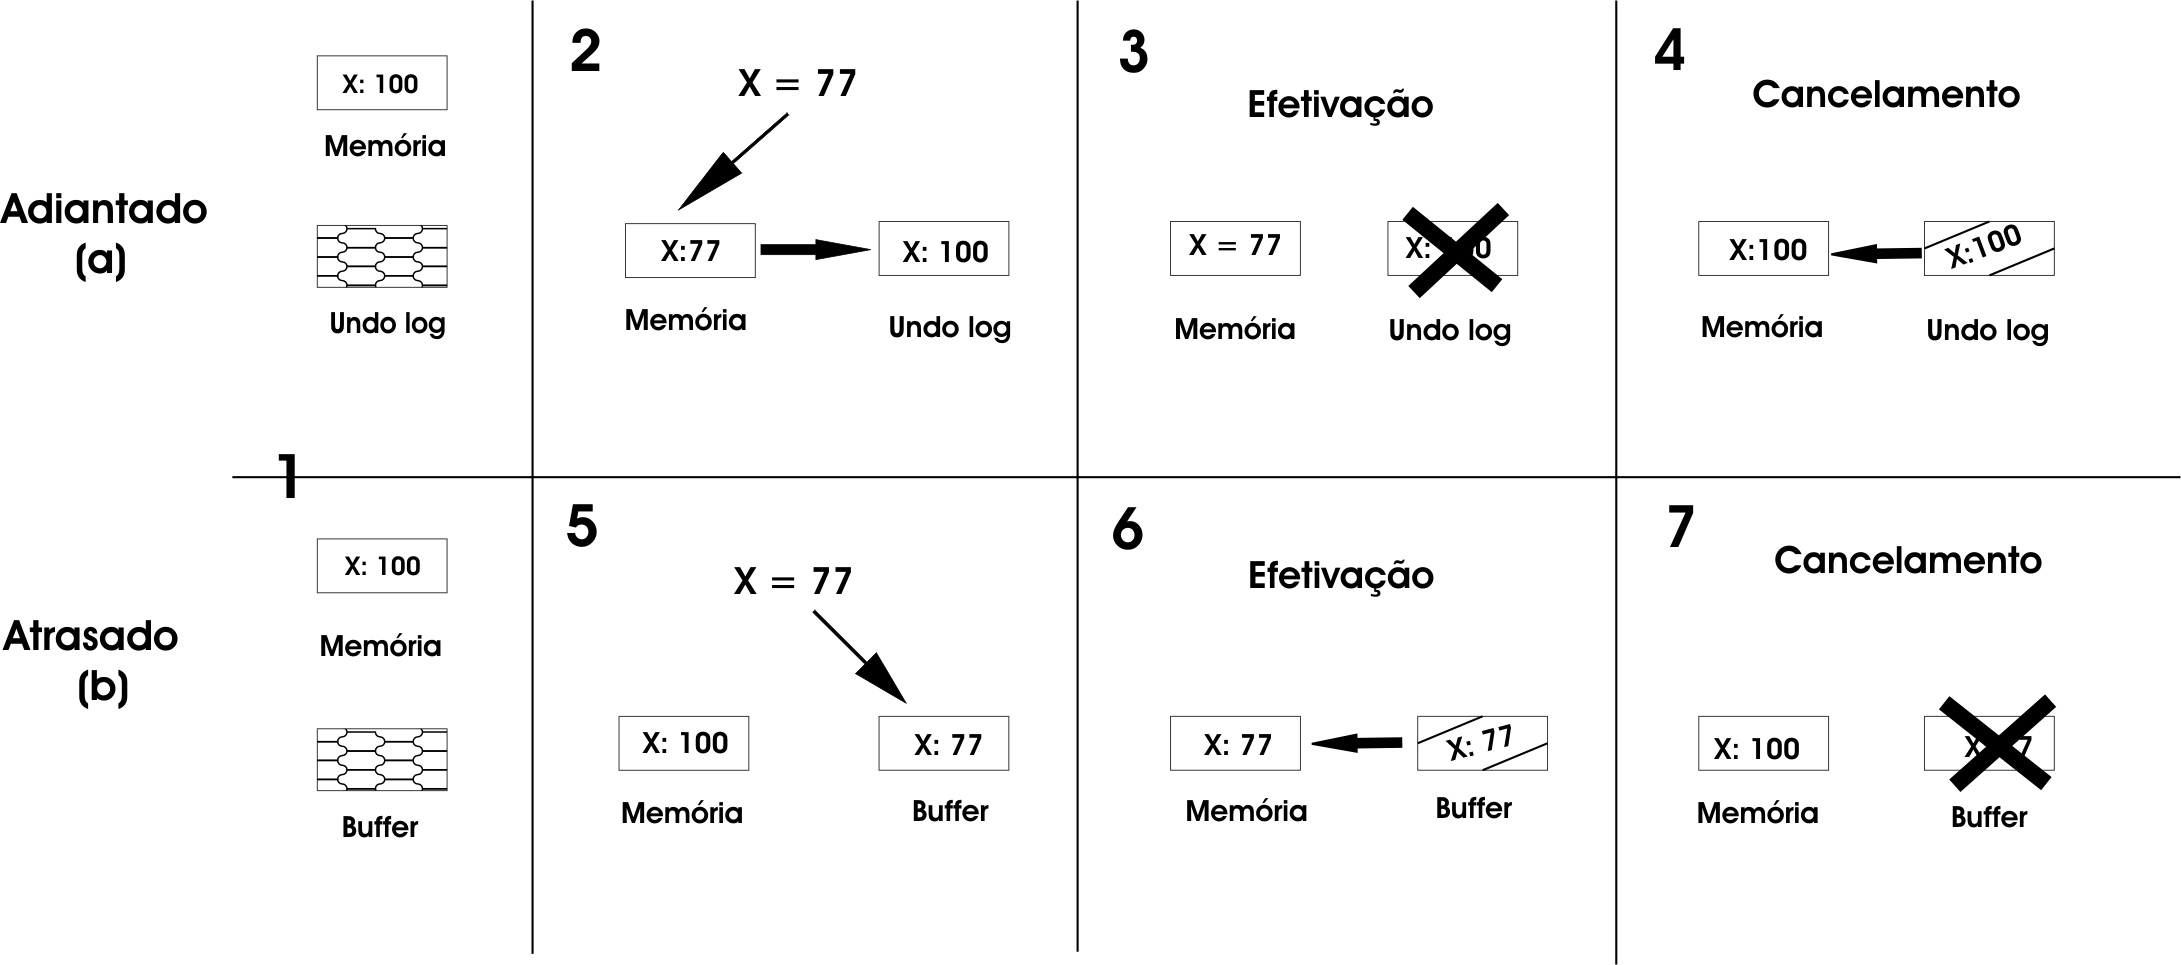
\includegraphics[height=7cm]{Imagens/versionamento.png}
\caption{Exemplo de versionamento adiantado (a) e atrasado (b). Fonte:~\cite{baldassinTese09}}
\label{figuraVersionamento}
\end{figure}

Existem dois tipos de versionamento de dados:

\begin{itemize}
 \item \textbf{Versionamento Adiantado}: como pode ser visto na Figura~\ref{figuraVersionamento}~(a), o valor modificado durante a transação é armazenado direto na memória e o valor inicial é armazenado em um \emph{undo log}, para que no caso de cancelamento na transação o valor inicial seja restaurado na memória.

 \item \textbf{Versionamento Atrasado}: como pode ser visto na Figura~\ref{figuraVersionamento}~(b) neste versionamento o valor modificado durante a transação é armazenado em um \emph{buffer} e o valor inicial é mantido na memória até que aconteça um \emph{commit} na transação, onde o valor armazenado no \emph{buffer} é escrito na memória. Caso aconteça o cancelamento na transação, o valor do \emph{buffer} é descartado.
\end{itemize}

%---------------------------------------------------------------------------------------------------%
\section{Detecção de Conflito}

Mecanismos de detecção de conflitos verificam a existência de operações conflitantes durante uma transação. Um conflito ocorre quando duas transações estão acessando um mesmo dado na memória e pelo menos uma das transações está fazendo uma operação de escrita~\cite{baldassinTese09}.

Da mesma forma que o versionamento de dados, a detecção de conflito também pode ser de dois tipos:

\begin{itemize}
 \item \textbf{Detecção de Conflitos Adiantado}: ocorrem no momento em que duas transações acessam um mesmo dado e uma delas faz uma operação de escrita. Essa operação de escrita é detectada e então uma transação é abortada. Neste tipo de detecção pode ocorrer o problema chamado de \emph{livelock}, quando duas transações ficam cancelando-se, desta forma, a execução do programa não progride. A Figura~\ref{figuradeteccaoadiantado} mostra como é feita a detecção de conflitos adiantado.

 O Caso~1, mostra a execução sem conflitos, onde as duas transações são executadas sem problemas. Já o Caso~2, mostra o que acontece quando ocorre um conflito, onde T1 lê A e logo depois T2 escreve em A, então o conflito é detectado e T1 é abortada, após ser efetivada T2, a transação T1 consegue ler A sem problema de conflito. Por fim o Caso~3 mostra a situação de \emph{livelock}, onde as duas transações tentam ler e escrever em A, assim as duas acabam sempre se abortando.

\begin{figure}[!htp]
\centering
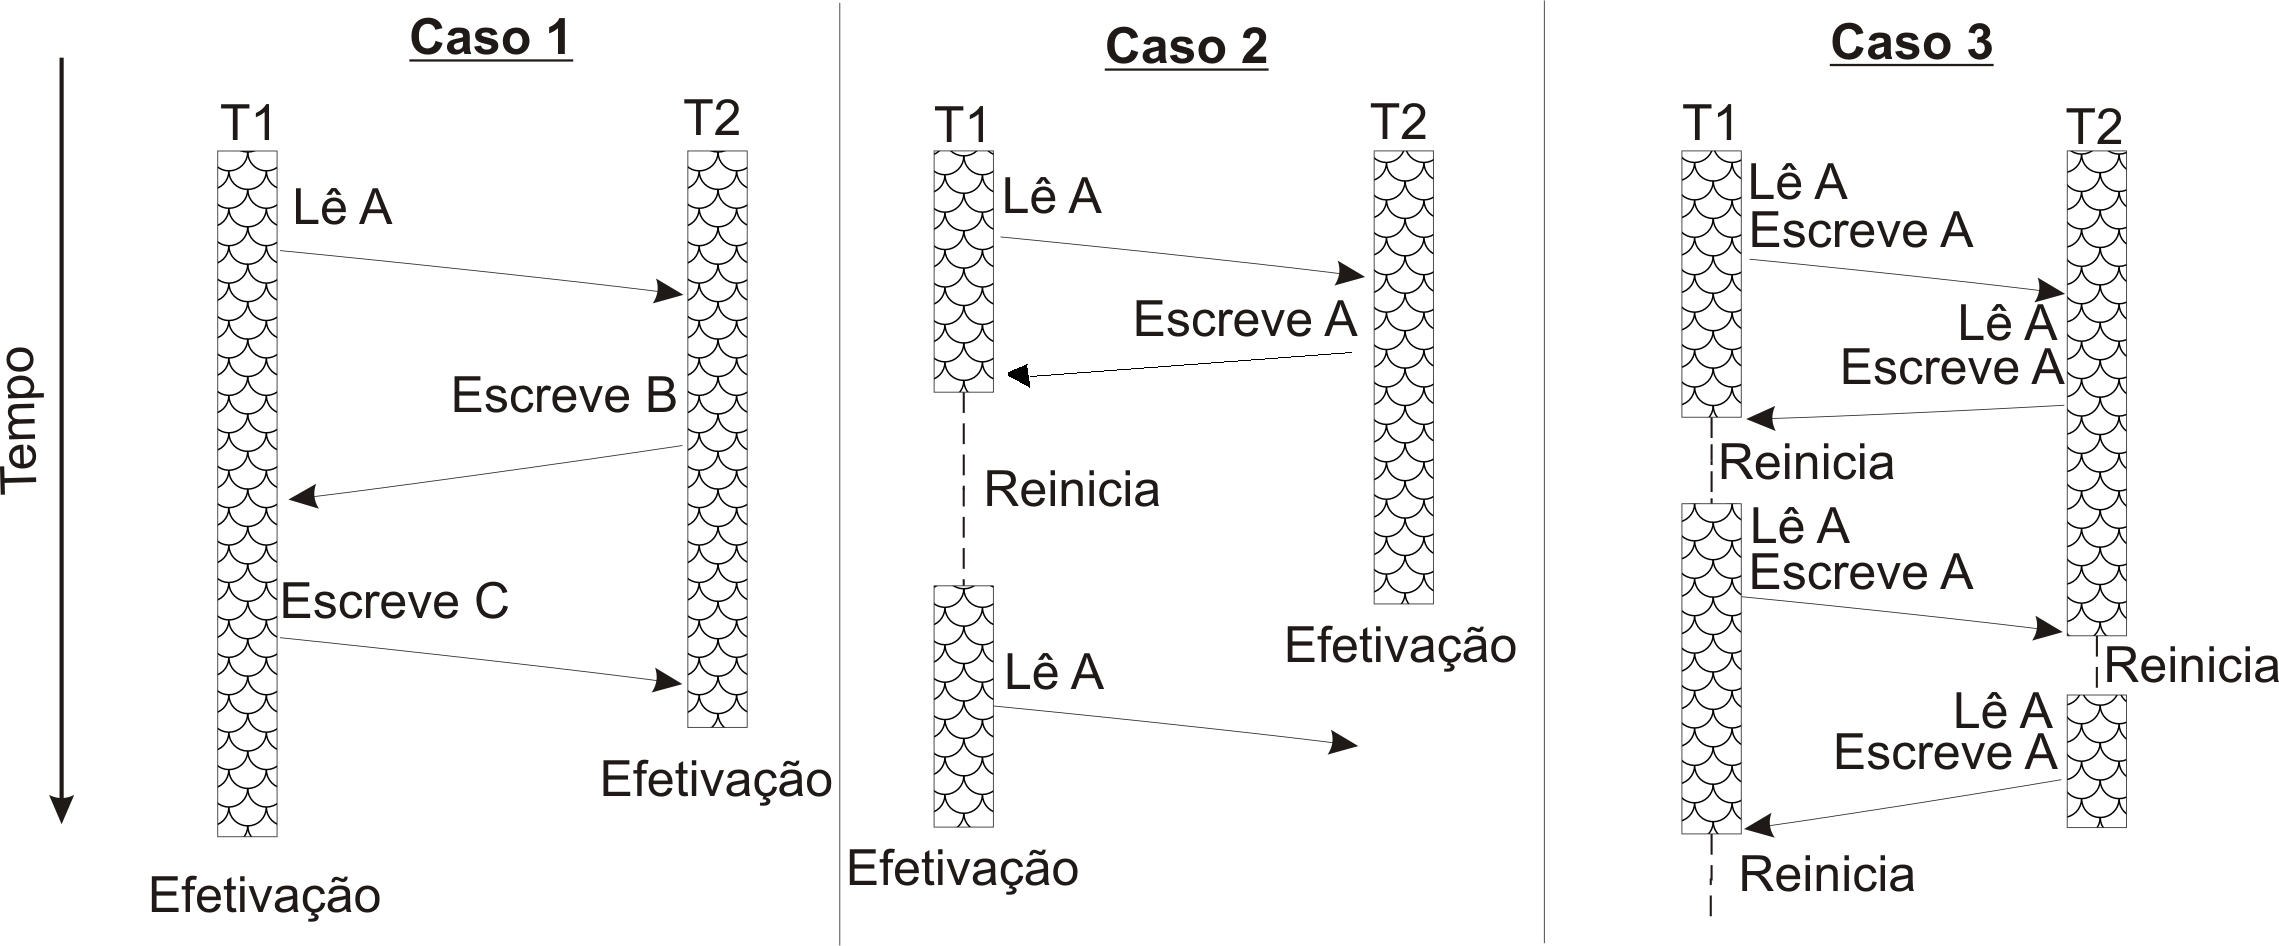
\includegraphics[height=6.5cm]{Imagens/conflitoadiantado.png}
\caption{Detecção de conflitos em modo adiantado. Fonte:~\cite{rigo07}}
\label{figuradeteccaoadiantado}
\end{figure}

 \item \textbf{Detecção de Conflitos Atrasado}: Este tipo de detecção de conflito ocorre no final da transação.  Antes da transação ser efetuada, é verificado se ocorreu um conflito. Caso tenha ocorrido, a transação é cancelada, senão é efetivada. Para transações muito grandes não é recomendado este tipo de detecção, pois uma transação grande pode ser abortada várias vezes por transações pequenas, assim gastando tempo de processamento desnecessário, este problema se chama \emph{starvation}. A Figura~\ref{figuradeteccaoatrasado} mostra como é feita a detecção de conflitos atrasado.

 O Caso~1, mostra as transações acessando dados diferentes, não ocasionando conflitos. No Caso~2, T2 lê A que é escrita por T1. A T2 só nota o conflito quando T1 é efetivado. Logo depois de notar o conflito T2 é abortada. No Caso~3 não ocorre nenhum conflito, pois T1 lê A antes de T2 escrever. O Caso~4 mostra a situação em que, após ser cancelada, T1 volta a executar.
\end{itemize}

\begin{figure}[!htp]
\centering
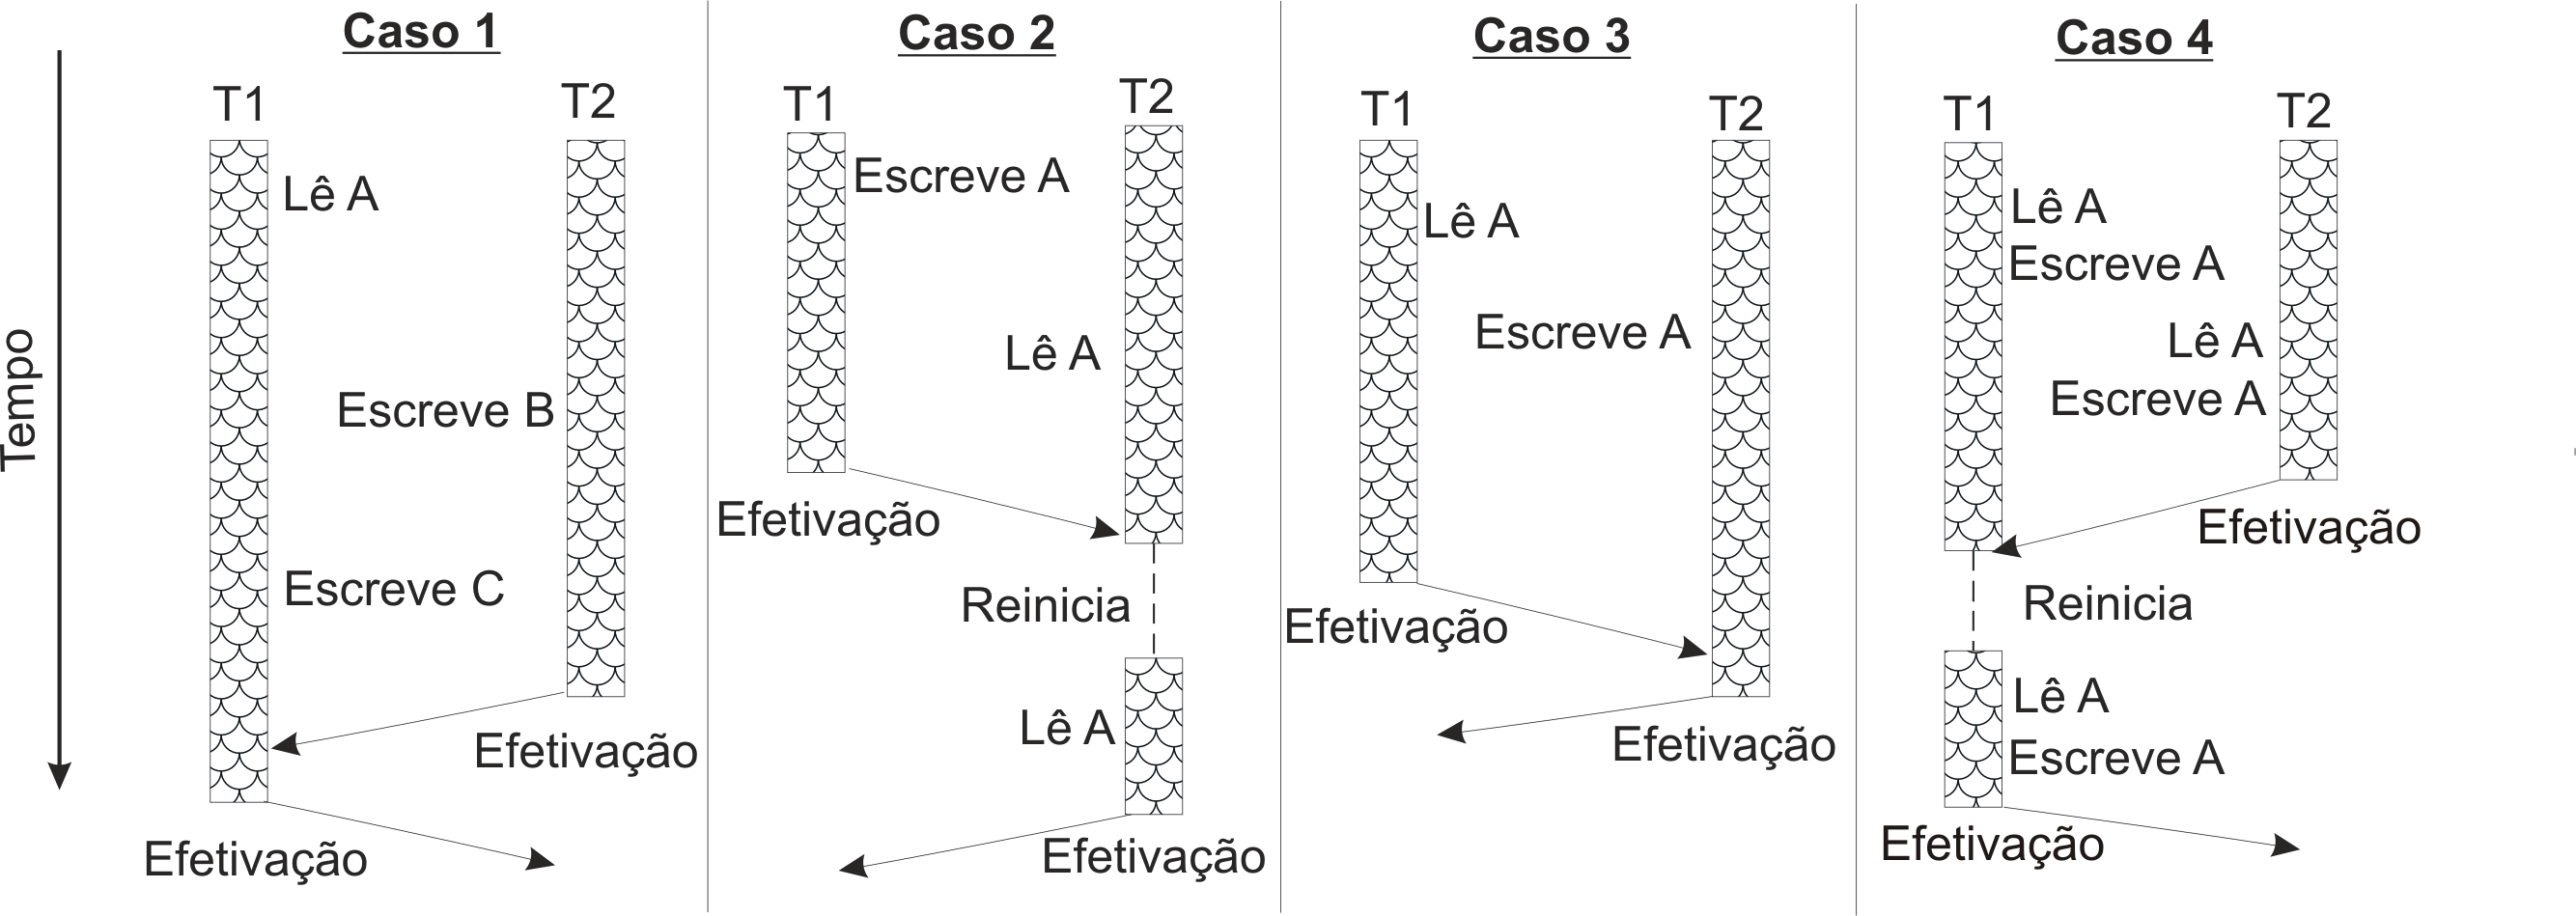
\includegraphics[height=6.5cm]{Imagens/conflitoatrasado.png}
\caption{Detecção de conflitos em modo atrasado. Fonte:~\cite{rigo07}}
\label{figuradeteccaoatrasado}
\end{figure}

Para solucionar o problema de qual transação continuará executando, quando ocorre um conflito, é utilizado um gerenciador de contenção~\cite{harris10}. O gerenciador de contenção é o responsável por decidir quando e qual transação vai ser abortada, isso para garantir que a execução do programa prossiga sem problemas.

%---------------------------------------------------------------------------------------------------%
%---------------------------------------------------------------------------------------------------%
\chapter{Escalonamento de Transações}

  ...


\chapter{Escalonadores NUMA}

  ...


\chapter{Escalonamento de Transações aplicado à NUMA}

  ...


\chapter{Discussões}

  ...


\chapter{Conclusão}

  ...

% Bibliografia
% http://liinwww.ira.uka.de/bibliography/index.html
% um site que cataloga no formato bibtex a bibliografia em computacao
%\bibliography{nomedoarquivo.bib} (sem extensao)
%\bibliographystyle{formato.bst} (sem extensao)

\bibliography{bibliografia}
\bibliographystyle{abnt}

% Anexos (Opcional)
\annex
\chapter{Um Anexo}

  ...

\end{document}
